\chapter{Future Work}
\label{Future Work}


This thesis was inspired by previous work that involved modeling a system that forecasted glucose in real time in patients with Type 2 Diabetes. Researchers utilized the Dual Unscented Kalman Filter for simultaneous state and parameter estimation \cite{article1}. The goal of this thesis was to create a similar model for Type 1 Diabetes (T1D). In previous work by \cite{Shtylla}, a 12 state mathematical model for T1D was developed. The relationship between these 12 states are shown in Figure ~\ref{fig:relations}

\begin{figure}[h]
    \centering
    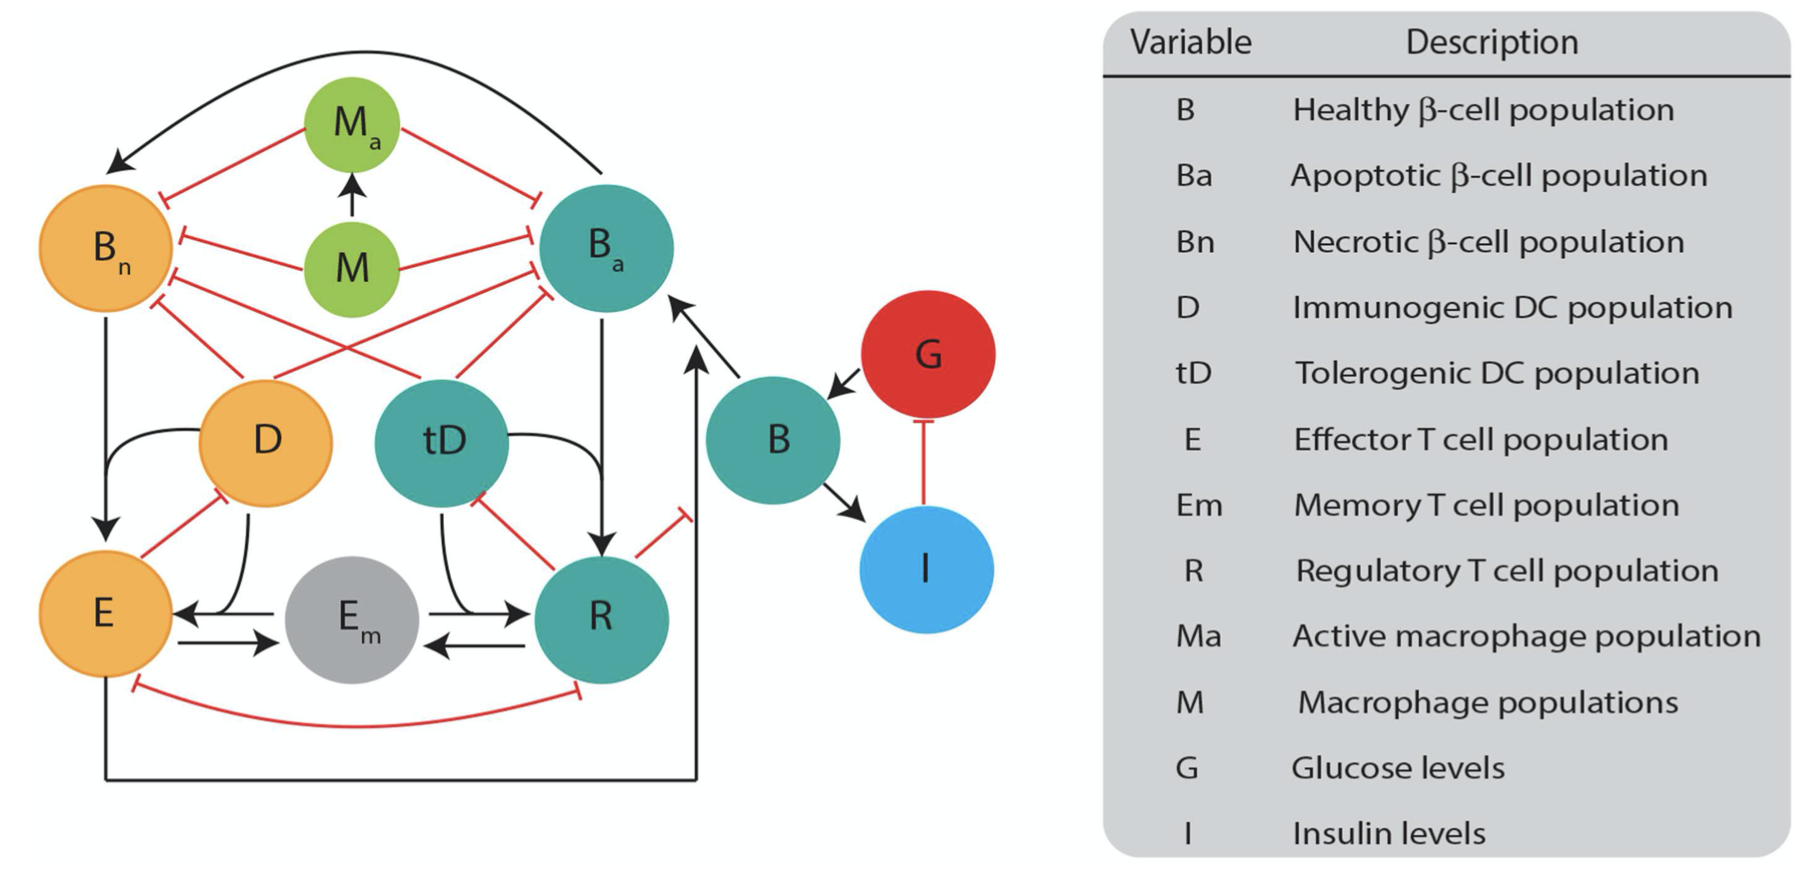
\includegraphics[scale = 0.5]{t1d_model.png}
    \caption{This image is taken from \cite{Shtylla} and provides a visualization on the relationships between the 12 states in this Type 1 Diabetes system.}
    \label{fig:relations}
\end{figure}

The 12 state system is given as 
\begin{align*}
    &\frac{d}{dt} G = R_0 - (G_0 + S_I I)G \\ 
    &\frac{d}{dt}  I = \sigma_1 K_1 (G, G_1) B - \delta_1 I \\
    &\frac{d}{dt} M = J +(k+b)M_a -cM - f_M MB_a - f_M MB_n - e_1M(M+M_a) \\
    & \frac{d}{dt} M_a = f_M MB_a +f_M MB_n - kM_a - e_2M_a(M + M_a) \\
    &\frac{d}{dt} B = \alpha_B K_1(G)B - \delta_B B - \eta_e(t)K_2(E,R)B - W(B, t)\\
    & \frac{d}{dt} B_a = \Tilde{\delta_B} + \Tilde{\eta_e} (t)K_2(E,R)B + \Tilde{W}(B, t) \\
    & \quad \quad  \quad \quad - dB_a - f_M MB_a - f_{M_a} B_a - f^{tD}(D_{SS} - D)B_a - f_D DB_a \\
    &\frac{d}{dt} B_n = dB_a - f_M MB_n - f_{M_a} M_a B_n - F_{Td}(D_{SS} - D)B_n - f_D DB_n \\
    & \frac{d}{dt} D = f_{tD}B_n(D_{SS} - D - tD) + f_{tD}B_n tD - b_{DE} ED - \mu_D D \\
    & \frac{d}{dt} tD = f_{tD}B_a(D_{SS} - D - tD) - f_{tD}B_n tD - b_{IR}RtD - \mu_D tD \\
    & \frac{d}{dt} E = a_E (T_{naive} - E) + b_p \frac{DE}{\theta_D + D} - r_{am}E + b_EDE_m - \mu_E ER \\
    & \frac{d}{dt} R = a_R (T_{naive} - R) + b_p \frac{tDR}{\theta_D + tD} - r_{am}R + b_R tDEm - \mu_R ER, \\
    & \frac{d}{dt} Em = r_{am}(E + R) - (a_{Em} + b_E D + b_R tD)eM
\end{align*}

\noindent \\ \\
\noindent Future direction includes utilizing parameter estimation techniques from this thesis and applying them to this system. Since this system has several more dimensions and is more complex than other systems considered in this thesis, results using the UKF will likely be better than that of the EKF. In addition, further study of alternative parameter estimation techniques, especially the Dual Unscented Kalman Filter, can be beneficial. \\ \\

